% Cita textual seccion Desarrolo:

% Deben explicarse los metodos numericos que utilizaron
% y su aplicacion al problema concreto involucrado en el trabajo practico.
% Se deben mencionar los pasos que siguieron para implementar
% los algoritmos, las dificultades que fueron encontrando y la
% descripcion de como las fueron resolviendo.

% Explicar tambien como fueron planteadas y realizadas las
% mediciones experimentales. Los ensayos fallidos, hipotesis y
% conjeturas equivocadas, experimentos y metodos malogrados deben
% figurar en esta seccion,
% con una breve explicacion de los motivos de estas fallas
% (en caso de ser conocidas).

% Template de matriz
% \[
% \begin{bmatrix} % Matriz con linea rectangular
% \begin{pmatrix} % Matriz con linea redonda
%     x_{11} & x_{12} & x_{13} & \dots  & x_{1n} \\
%     x_{21} & x_{22} & x_{23} & \dots  & x_{2n} \\
%     \vdots & \vdots & \vdots & \ddots & \vdots \\
%     x_{d1} & x_{d2} & x_{d3} & \dots  & x_{dn}
% \end{pmatrix}
% \end{bmatrix}
% \]

\section{Calibración}

Queremos calcular las normales en cada punto de la superficie.
Tomando 3 imagenes diferentes (por ej 1, 2 y 3), utilizamos las luces $s_{algo}$ y las intensidades registradas $I_{algo}$ para calcular los $m_{algo}$ que son $tal cosa$.
\todo[inline]{mejorar intro}
Los $I_{algo}$ podemos obtenerlos $asi y asa$, que es sencillo. No es tan trivial el calculo de los $s_{algo}^{i}$.

Es decir, necesitamos resolver el siguiente sistema: \\

\[
% \begin{bmatrix} % Matriz con linea rectangular
\begin{pmatrix}
    s_{x}^{1} & s_{y}^{1} & s_{z}^{1} \\
    s_{x}^{2} & s_{y}^{2} & s_{z}^{2} \\
    s_{x}^{3} & s_{y}^{3} & s_{z}^{3}
\end{pmatrix}
% \end{bmatrix}
\begin{pmatrix}
    m_{x} \\
    m_{y} \\
    m_{z}
\end{pmatrix}
=
\begin{pmatrix}
    I_{1} \\
    I_{2} \\
    I_{3}
\end{pmatrix}
\]


Tenemos que $S = (s_{x}^{i}, s_{y}^{i}, s_{z}^{i})$ es el vector luz en la imagen $i$. Dado que vamos a explicar el cálculo para una imagen cualquiera, omitiremos el supraíndice $i$ para una notación mas relajada.

Llamemos $c = (c_{x}, c_{y}, c_{z})$ al centro de la esfera. Pensemos la luz como un vector que apunta hacia el centro. El vector $S$ toca la superficie en un cierto punto $p = (p_{x}, p_{y}, p_{z})$, pero $p$ no es un punto al azar, sino que es el punto más iluminado de la esfera. Por lo tanto, la dirección de luz que nos interesa es $S =  c - p$.\\

{\centering
    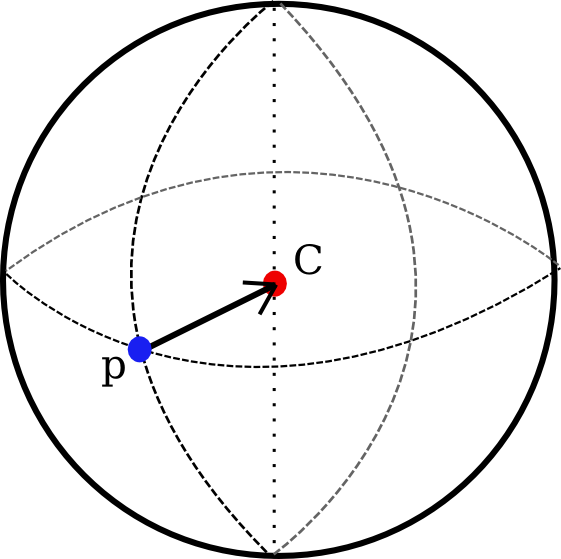
\includegraphics[scale=0.9]{informe/imagenes/esfera/esferaModelo.png} \\
    \captionof{figure}{Vemos que el vector que nos interesa es $S = c - p$}
}

$ $\newline

Mas precisamente, $S = (c_{x} - p_{x}, c_{y} - p_{y}, c_{z} - p_{z}).$ En principio no conocemos ninguno de estos valores, pero concentrémonos en calcular sobre el eje $x$ e $y$. De la imagen de la esfera (2D) podemos conocer algunos datos. En la implementación utilizamos la máscara provista por la cátedra para simplificar los cálculos. \\

Como los píxeles en la máscara son blancos o negros, es muy sencillo identificar los puntos que pertenecen a la esfera con sólo ver su color. Recorriendo todos los puntos y tomando máximos y mínimos obtenemos 4 puntos clave: El punto del círculo que está mas a arriba $A$, el más abajo $A'$, el de más a la izquierda $B$ y el de más a la derecha $B'$. \\

{\centering
    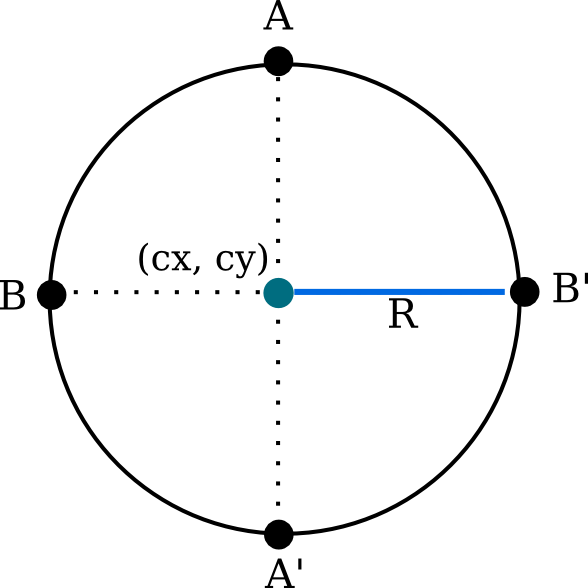
\includegraphics[scale=0.5]{informe/imagenes/esfera/circulo.png} \\
}

Puede verse fácilmente que el radio $R$ del círculo es la mitad de la distancia entre $B$ y $B'$

\begin{center}
$R = \frac{|B'_x - B_x|}{2}$.
\end{center}

Además, sabiendo que $c$ es el centro del círculo,

\begin{center}
    $c_{x} = B_x + R$ \\
    $c_{y} = A_y + R$
\end{center}




\section{Métodos}

\subsection{Eliminación Gaussiana}

\todo[inline]{Hablar del algoritmo}
\todo[inline]{Explicar por que podemos aplicarlo con las luces, decir que las 3 que tomamos son li entonces no pincha nunca}

\subsection{LU}
\todo[inline]{Que es esto}
\todo[inline]{Por que nos sirve para nuestro problema, hablar de repeticion de calculos}

\subsection{Cholesky}
\todo[inline]{algo}


\section{Cálculo de normales}

\todo[inline]{Explicar que es lo que tenemos que resolver}
\todo[inline]{Explicar como aplicamos los metodos listados arriba para resolver el problema, y por que podemos hacerlo}


\section{Estimacion de profundidades}

\todo[inline]{Hablar del ultimo sistema de ecuaciones de la cual (aun) no tengo idea}


\section{Resultados}
\todo[inline] {Dar imagenes minimo del resultado final}



\section{Experimentación}

\todo[inline]{PENSAR MAS}
\todo[inline]{Mostrar como con diferentes luces obtenemos diferentes normales}
\todo[inline]{Diferencias de tiempos EG vs LU vs mascara y combinaciones}

